\section{Experiments}
\label{sec:exp}
In this section, we first describe the dataset used in our paper. We then introduce all baselines, evaluation metric, and setting. Finally, we present our research questions and results.

\subsection{Dataset}
\label{sec:dataset}
\cmt{TODO: add the information about the dataset}

\subsection{Baseline}
\label{sec:baseline}

We compare our proposed model with the Just-in-Time (JIT) defect prediction approach mentioned in~\cite{mcintosh2018fix}. Different from the JIT model used to identify fix-inducing code changes, we train the model to identify bugs. We also use a nonlinear variant of multiple regression modeling to fit the JIT model. The nonlinear regression modeling has widely used in software engineering to understand the relationship between software development practices and software quality~\cite{zhou2011does, morales2015code, mcintosh2016empirical}. 

\subsection{Training and hyperparameters}
\label{sec:training_parameters}

%We empirically run PatchNet on different the number of convolutional filters and number of convolutional filter length and select the best number of convolutional filters and filter length for our model. %(i.e., $k=1$ and $k=2$) having length 64 on both \textit{commit message module} and \textit{commit code module} for training PatchNet. 

% PatchNet also has a number of other hyperparameters. 
% We set the size of PatchNet's hidden layer ($\textbf{h}$), $l_2$ regularization, and the dropout rate to be 100, $1e-5$, and 0.5, respectively. The dimensions of
% the word vectors in commit message $d_m$ and code changes $d_c$ are set to
% 50. PatchNet is trained using SGD~\cite{bottou2010large} with shuffled
% mini-batches. The batch size is set to 32. We train PatchNet for 25 epochs
% and apply the early stopping strategy~\cite{prechelt1998automatic}, i.e.,
% we stop the training if there has been no update to the loss value (see Equation~\ref{eq:cost}) for the last 5 epochs. These parameters follow a prior work~\cite{severyn2015learning}. 

% The parameters \jl{hyperparameters?} of PatchNet were chosen as follows:
% the number of convolutional filters, the size of PatchNet's hidden layer
% ($\textbf{h}$), $l_2$ regularization \jl{I don't understand what is the
%   parameter here}, and the dropout rate to be 64, 100, $1e-5$, and 0.5,
% respectively \jl{This is hard to read - the respectively is too complex.
%   Just give the numbers one by one.  Or consider making a table.}. The
% dimensions of the word vectors in commit message $d_m$ and code changes
% $d_c$ are set to 50. PatchNet is trained using SGD~\cite{bottou2010large}
% \jl{I thought we use Adam, which is different than SGD.} with shuffled
% mini-batches. The batch size is set to 32. We train PatchNet for 25 epochs
% and apply the early stopping strategy~\cite{prechelt1998automatic}, i.e.,
% we stop the training if there has been no update to the loss value (see
% Equation~\ref{eq:cost}) for the last 5 epochs. All these parameters of our
% model are in line with a prior work~\cite{severyn2015learning, yu2014deep}.

% \jh{Comment 8: Hyper-parameters: how do we select parameters for deep learning models? (reviewer C, meta reviewer)}

% \jg{Julia: can you please check this section?}

For the size of the convolutional filters, we choose 64. The size of DeepJIT's fully-connected layer described in Section~\ref{sec:ftr_combine} is set to 512. The word vectors dimension of the commit message ($d_m$) and code changes ($d_c$) are set to 64. We train DeepJIT using Adam~\cite{kingma2014adam} with shuffled mini-batches.  The batch size is set to 32. We train DeepJIT for 100 epochs. We also apply the early stopping strategy~\cite{prechelt1998automatic, caruana2001overfitting} to avoid overfitting problem during the training process. Typically, we stop the training if the value of the objective function (see Equation~\ref{eq:cost}) has been no update in the last 5 epochs. All these hyperparameters in our paper are widely used in the deep learning community~\cite{severyn2015learning, huo2016learning, huo2017enhancing, hinton2012improving}. 
 

\subsection{Evaluation Metric and Setting}
\label{sec:metric_setting}

\subsection{Research Questions and Results}
\label{sec:rq_results}

\noindent \textbf{RQ1: How effective is our proposed deep learning model compared to the state-of-the-art baseline?}

\begin{figure}
\center
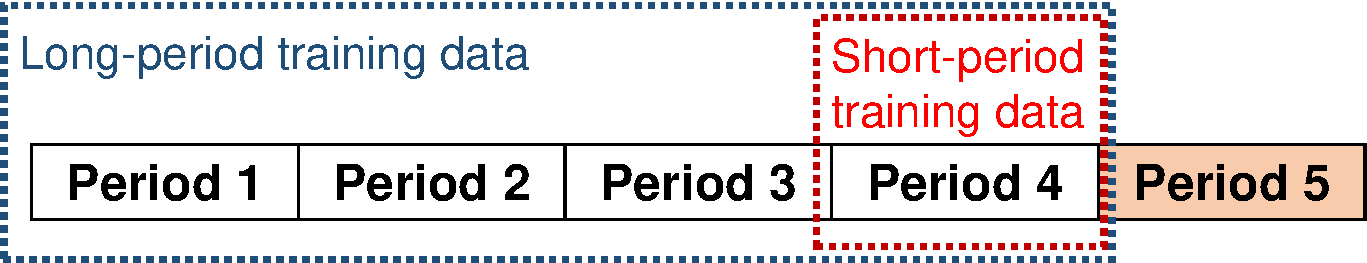
\includegraphics[scale=0.36]{figs/split.pdf}
\caption{An example of choosing the data for training proposed model. The last period will be used as testing data.}
\label{fig:splitting}
\end{figure}

\begin{table*}[t!]
  \centering
  \caption{The AUC results of DeepJIT vs. with other baselines in three settings: short-period, long-period, and random}
    \begin{tabular}{|l|c|c|c|c|c|c|}
    \hline
    \multirow{2}[4]{*}{} & \multicolumn{3}{c|}{QT} & \multicolumn{3}{c|}{OPENSTACK} \\
\cline{2-7}          & \multicolumn{1}{l|}{Short-Period} & \multicolumn{1}{l|}{Long-period} & \multicolumn{1}{l|}{Random} & \multicolumn{1}{l|}{Short-Period} & \multicolumn{1}{l|}{Long-period} & \multicolumn{1}{l|}{Random} \\
    \hline
    \hline
    JIT   & 0.703 & 0.702 & 0.701 & 0.711 & 0.706 & 0.691 \\
    \hline
    DBNJIT & 0.714 & 0.708 & 0.705 & 0.716 & 0.712 & 0.694 \\
    \hline
    DeepJIT & \textbf{0.764} & \textbf{0.765} & \textbf{0.768} & \textbf{0.781} & \textbf{0.771} & \textbf{0.751} \\
    \hline
    \end{tabular}%
  \label{tab:results}%
\end{table*}%

\noindent \textbf{RQ2: Does the proposed model benefit both commit message and the code changes?}

\begin{table*}[t!]
  \centering
  \caption{Contribution of feature components in DeepJIT}
    \begin{tabular}{|l|c|c|c|c|c|c|}
    \hline
    \multirow{2}[4]{*}{} & \multicolumn{3}{c|}{QT} & \multicolumn{3}{c|}{OPENSTACK} \\
\cline{2-7}          & \multicolumn{1}{l|}{Short-Period} & \multicolumn{1}{l|}{Long-period} & \multicolumn{1}{l|}{Random} & \multicolumn{1}{l|}{Short-Period} & \multicolumn{1}{l|}{Long-period} & \multicolumn{1}{l|}{Random} \\
    \hline
    \hline
    DeepJIT-Msg & 0.609 & 0.638 & 0.641 & 0.583 & 0.659 & 0.689 \\
    \hline
    DeepJIT-Code & 0.734 & 0.727 & 0.738 & 0.769 & 0.738 & 0.729 \\
    \hline
    DeepJIT & \textbf{0.764} & \textbf{0.765} & \textbf{0.768} & \textbf{0.781} & \textbf{0.771} \\
    \hline
    \end{tabular}%
  \label{tab:variants}%
\end{table*}%

\noindent \textbf{RQ3: Does the proposed model benefit from the manually extracted code changes features?}

\begin{table*}[t!]
  \centering
  \caption{Combination of DeepJIT with JIT's features}
    \begin{tabular}{|l|c|c|c|c|c|c|}
    \hline
    \multirow{2}[4]{*}{} & \multicolumn{3}{c|}{QT} & \multicolumn{3}{c|}{OPENSTACK} \\
\cline{2-7}          & Short-Period & Long-period & Random & Short-Period & Long-period & Random \\
    \hline
    \hline
    DeepJIT & 0.764 & 0.765 & 0.768 & 0.781 & 0.771 & 0.751 \\
    \hline
    DeepJIT-Combined & \textbf{0.788} & \textbf{0.786} & \textbf{0.779} & \textbf{0.814} & \textbf{0.799} & \text{0.760} \\
    \hline
    \end{tabular}%
  \label{tab:combined}%
\end{table*}%

\noindent \textbf{RQ4: How are the time costs of the proposed model?}


